%
% thomas.tex
%
% (c) 2020 Prof Dr Andreas Müller, Hochschule Rapperswil
%
\section{Direkte Verfahren
\label{buch:section:direkt}}
\rhead{Direkte Verfahren}
Das primäre direkte Verfahren zur Lösung linearer Gleichungssysteme ist
der Gauss-Algorithmus, der allerdings
zur Lösung linearer Gleichungssysteme im Allgemeinen $O(n^3)$
Operationen braucht, was für grosse $n$ zu aufwendig ist.
\index{Gauss-Algorithmus}%

%
% XXX Formelzusammenstellung für den Gauss-Algorithmus
%

\subsection{Thomas-Algorithmus für tridiagonale Matrizen
\label{buch:subsection:thomasalgorithmus}}
Es gibt einen Fall, der zum Beispiel bei der Diskretisierung
partieller Differentialgleichungen mit nur einer Raumdimension
häufig auftritt, nämlich der Fall {\em tridiagonaler} Koeffizientenmatrix.
\index{tridiagonal}
Dies sind Matrizen der Form
\begin{equation}
A
=
\begin{pmatrix}
b_1   & c_1   &  0    &  0    &\dots  &  0    &  0     \\
a_2   & b_2   & c_2   &  0    &\dots  &  0    &  0     \\
 0    & a_3   & b_3   & c_3   &\dots  &  0    &  0     \\
 0    &  0    & a_4   & b_4   &\ddots &  0    &  0     \\
\vdots&\vdots &\vdots &\ddots &\ddots &\ddots &\vdots  \\
 0    &  0    &  0    &  0    &\ddots &b_{n-1}&c_{n-1} \\
 0    &  0    &  0    &  0    &\dots  &a_{n}  &b_n
\end{pmatrix},
\end{equation}
deren Einträge alle $0$ sind ausser auf der Diagonalen und den unmittelbar
benachbarten Nebendiagonalen.
\index{Nebendiagonale}%
Eine solche Matrix enstand auch im
Abschnitt~\ref{buch:subsection:splineinterpolant}
bei der Bestimmung der Steigungen für die Spline-Interpolationsfunktion.
\index{Spline-Interpolationsfunktion}%

Da die meisten Einträge der Matrix verschwinden, geben nur die wenigstens
Zeilenoperationen des Gauss-Algorithmus überhaupt etwas zu tun.
Dadurch sinkt der Aufwand für die Durchführung des Algorithmus.
\index{Gauss-Algorithmus}%
\index{Zeilenoperation}%

\subsubsection{Vorwärtsreduktion}
Die Vorwärtsreduktion entfernt die Element unter der Diagonalen
und macht die Pivotelemente zu $1$.
\index{Vorwärtsreduktion}%
\index{Pivotelement}%
Man muss also nur herausfinden, wie sich die Elemente $c_i$ über der
Diagonalen verändern.
Bei der Vorwärtsreduktion wird das ursprüngliche Gauss-Tableau daher
wie folgt umgewandelt:
\index{Gauss-Tableau}%
\[
\begin{tabular}{|>{$}c<{$}>{$}c<{$}>{$}c<{$}>{$}c<{$}>{$}c<{$}>{$}c<{$}|>{$}c<{$}|}
\hline
b_1   & c_1  &  0   &  0   &  0   &\dots & d_1  \\
a_2   & b_2  & c_2  &  0   &  0   &\dots & d_2  \\
 0    & a_3  & b_3  & c_3  &  0   &\dots & d_3  \\
 0    &  0   & a_4  & b_4  & c_4  &\dots & d_4  \\
\vdots&\vdots&\vdots&\vdots&\vdots&\ddots&\vdots\\
\hline
\end{tabular}
\to
\begin{tabular}{|>{$}c<{$}>{$}c<{$}>{$}c<{$}>{$}c<{$}>{$}c<{$}>{$}c<{$}|>{$}c<{$}|}
\hline
 1    & c_1' &  0   &  0   &  0   &\dots & d_1' \\
 0    &  1   & c_2' &  0   &  0   &\dots & d_2' \\
 0    &  0   &  1   & c_3' &  0   &\dots & d_3' \\
 0    &  0   &  0   &  1   & c_4' &\dots & d_4' \\
\vdots&\vdots&\vdots&\vdots&\vdots&\ddots&\vdots\\
\hline
\end{tabular}
\]
mit
\begin{equation}
c_i
=
\begin{cases} 
\displaystyle \frac{c_1\mathstrut}{b_1\mathstrut}            &\quad i=1\\[8pt]
\displaystyle \frac{c_i\mathstrut}{b_i-a_ic'_{i-1}\mathstrut}&\quad i>1
\end{cases}
\qquad\text{und}\qquad
d_i
=
\begin{cases}
\displaystyle\frac{d_1\mathstrut}{b_1\mathstrut}                        &\quad i=1\\[8pt]
\displaystyle\frac{d_i-a_id'_{i-1}\mathstrut}{b_i-a_ic'_{i-1}\mathstrut}&\quad i>1
\end{cases}
\label{buch:equation:thomasvorwaerts}
\end{equation}
Die Vorwärtsreduktion ist also mit $O(n)$ Operationen durchführbar.

\begin{beispiel}
In der Matrix
\begin{equation}
A=\begin{pmatrix}
    -2&     1&     0&     0&     0&\dots \\
     1&    -2&     1&     0&     0&\dots \\
     0&     1&    -2&     1&     0&\dots \\
     0&     0&     1&    -2&     1&\dots \\
     0&     0&     0&     1&    -2&\ddots\\
\vdots&\vdots&\vdots&\vdots&\ddots&\ddots
\end{pmatrix}
\label{buch:equation:Atridiagonal}
\end{equation}
gilt $a_i=1$, $b_i=-2$ und $c_i=1$ für alle $i$.
Aus den Formeln~\eqref{buch:equation:thomasvorwaerts}
folgt dann
\begin{align*}
c_1'&=-\frac12
\\
c_2'&=\frac{1}{-2-c_1'}=\frac{1}{-2+\frac12}=-\frac{2}{3}
\\
c_3'&=\frac{1}{-2-c_2'}=\frac{1}{-2+\frac{2}{3}}=\frac{3}{-2\cdot 3 + 2}
=-\frac{3}{4}.
\end{align*}
Daraus lässt sich vermuten, dass
\begin{equation}
c_k'=-\frac{k}{k+1}
\label{buch:equation:ck}
\end{equation}
gilt.
Tatsächlich lässt sich dies mit vollständiger Induktion beweisen.
\index{vollständige Induktion}%
Zunächst ist $c_1=-\frac12=-\frac1{1+1}$ korrekt.
Jetzt muss man zeigen, dass aus der Formel \eqref{buch:equation:ck} für $k$
die Formel für $k+1$ folgt.
Durch nachrechnen sieht man, dass
\[
c_{k+1}'
=
\frac1{-2-c_{k}'}
=
\frac{1}{-2+\displaystyle\frac{k}{k+1}}
=
\frac{k+1}{-2(k+1)+k}
=
-\frac{k+1}{k+2}.
\]
Damit ist \eqref{buch:equation:ck} bewiesen.

Wir führen die Vorwärtsreduktion für einen Vektor aus lauter Einsen
als rechte Seite durch, also $d_i=1$.
\index{Vorwärtsreduktion}%
Die Formeln \eqref{buch:equation:thomasvorwaerts} gibt dann
\begin{align*}
d_1'
&=
\frac{d_1}{b_1} = -\frac12
\\
d_2'
&=
\frac{1-d_1'}{-2-c_1'}
=
\frac{\frac32}{-2+\frac12}
=
\frac{\frac32}{-\frac{3}{2}}
=-1
\\
d_3'
&=
\frac{1-d_2'}{-2+c_2'}
=
\frac{1+1}{-2+\frac23}
=
\frac{2\cdot 3}{-2\cdot 3 + 2}
=
-\frac{3}{2}.
\end{align*}
Aus diesen Werten lässt sich wieder die Vermutung 
\[
d_{k}'=-\frac{k}2
\]
ableiten.
Und tatsächlich beweist die Rechnung
\[
d_{k+1}'
=
\frac{1-d_k'}{-2+\frac{k}{k+1}}
=
\frac{1+\frac{k}{2}}{-2+\frac{k}{k+1}}
=
\frac{1+\frac{k}{2}}{-2(k+1)+k} (k+1)
=
\frac{k+2}{-2k-2+k}
\cdot
\frac{k+1}{2}
=
\frac{k+2}{-k-2}
\cdot
\frac{k+1}{2}
=
-\frac{k+1}{2}
\]
diese Vermutung mit vollständiger Induktion.
\end{beispiel}

\subsubsection{Rückwärtseinsetzen}
\index{Rückwärtseinsetzen}%
Das Rückwärtseinsetzen ist jetzt ebenfalls sehr einfach:
\begin{equation}
x_k = \begin{cases}
d_n'&\quad k=n
\\
d_k'  - c_k' x_{k+1} &\quad k < n
\end{cases}
\label{buch:equation:rueckwaerts}
\end{equation}
Auch das Rückwärtseinsetzen ist daher mit $O(n)$ Operationen machbar.
Der Thomas-Algorithmus löst also ein tridiagonales Gleichungssystem in
\index{Thomas-Algorithmus}%
$O(n)$ Operationen oder berechnet die inverse Matrix einer 
tridiagonalen Matrix in $O(n^2)$ Operationen.

\begin{beispiel}
Für die Matrix $A$ von \eqref{buch:equation:Atridiagonal} und die rechte
Seite von Einsen aus dem entsprechenden Beispiel  können wir jetzt auch
das Rückwärtseinsetzen durchführen.
Dazu wenden wir die Formeln
\eqref{buch:equation:rueckwaerts}
auf die oben gefundenen Werte $c'_k=-k/(k+1)$ und $d_k'=-k/2$ an und
erhalten
\begin{align*}
x_n
&=
-\frac{n}{2}
&&=\frac{1\cdot (n-0)}2
\\
x_{n-1}
&=
-\frac{n-1}{2} -\biggl(-\frac{n-1}{n}\biggr)\cdot \biggl(-\frac{n}2\biggr)
=
-\frac{n-1}{2} - \frac{n-1}{2}
=
-(n-1)
&&=-\frac{2(n-1)}{2}
\\
x_{n-2}
&=
-\frac{n-2}{2} - \biggl(-\frac{n-2}{n-1}\biggr) \cdot (-n+1)
=
-\frac{n-2}{2} - (n-2)
=
-\frac{3(n-2)}2
&&=-\frac{3(n-2)}2
\\
x_{n-3}
&=
-\frac{n-3}{2} - \frac{n-3}{n-2} \frac{3(n-2)}2
=
-\frac{n-3}{2} - 3\frac{n-3}2
=
\frac{4(n-3)}2
&&=-\frac{4(n-3)}2
\end{align*}
woraus man die Vermutung
\begin{equation}
x_{n-k} = -\frac{(k+1)(n-k)}2
\label{buch:equation:xn}
\end{equation}
ableiten.
Tatsächlich rechnet man nach
\begin{align*}
x_{n-(k+1)}
=
d_{n-(k+1)}'-c_{n-(k+1)}'x_{n-k}
&=
-\frac{n-(k+1)}2-\frac{n-k-1}{n-k}\cdot \frac{(k+1)(n-k)}2
\\
&=
-\frac{n-(k+1)+(n-k-1)(k+1)}2
\\
&=
-\frac{(k+2)(n-(k+1))}2.
\end{align*}
Damit ist die Formel für $x_n$ bewiesen.

Man kann natürlich auch direkt verifizieren, dass die $x_k$ das tridiagonale
Gleichungssystem lösen:
\begin{align*}
x_{n-(k-1)}-2x_{n-k} + x_{n-(k+1)}
&=
-\frac{
k(n-(k-1))
-2(k+1)(n-k)
+(k+2)(n-(k+1))
}2
\\
&=
-\frac{
kn-k^2+k
-2kn-2n+2k^2+2k
+kn+2n-k^2-3k-2}2=1.
\end{align*}
Dies gilt auch für $k=0$  und $k=n-1$, weil die Formel~\eqref{buch:equation:xn}
\[
x_{n+1}=x_{n-(-1)} = -\frac{(-1+1)(n-(-1))}2=0
\qquad\text{und}\qquad
x_0 = x_{n-n} = -\frac{(n+1)(n-n)}2
\]
zur Folge hat.
\end{beispiel}

\subsection{Zyklisch tridiagonale Matrix
\label{buch:subsection:zyklischtridiagonal}}
Die Diskretisation des Poisson-Problems oder der Wärmeleitungsgleichung
auf einem Ring liefert eine tridiagonale Matrix, in der zusätzlich die
Einträge in den Ecken links unten und rechts oben von $0$ verschieden sind.
\index{Poisson-Problem}%
\index{Matrix!tridiagonal}%
\index{tridiagonale Matrix}%
Bei der Durchführung des Gauss-Algorithmus werden damit zusätzliche 
Einträge im Tableau von $0$ verschieden sein, so dass zusätzliche Operationen
notwendig werden:
\index{Gauss-Algorithmus}%
\index{Tableau}%
\begin{itemize}
\item 
Zusätzlich zu der Zeilenoperation, die die Element 
$a_i$ zu $0$ macht braucht es jeweils noch eine Operation, welche das
Element in der letzten Zeile annihiliert.
\index{Zeilenoperation}%
Dadurch wird aber ein neuer nicht verschwindender Eintrag erzeugt,
so dass eine Operation für jedes Element der letzten Zeile nötig wird,
also $O(n)$ zusätzliche Operation.
\item
Die Zeilenoperationen erzeugen aus dem Element in der rechten oberen
Ecke nicht verschwindende Elemente in der Spalte ganz recht.
Beim Rückwärtseinsetzen sind daher im ersten Schritt $O(n)$ 
zusätzliche Operatione notwendig.
\end{itemize}
Auch ein Gleichungssystem mit zyklisch tridiagonaler Matrix lässt sich also 
mit $O(n)$ Operationen lösen und die Matrix lässt sich mit $O(n^2)$
Operationen invertieren.

Tatsächlich erfordert das Invertieren einer Matrix nur $O(n^2)$
zusätzliche Operationen, wenn die Inverse einer Matrix bereits
bekannt ist, die sich in nur einer Stelle unterscheidet.
Dies ist der Inhalt der Sherman-Morrison-Woodbury-Formel, die
im nächsten Abschnitt untersucht wird.

\subsection{Sherman-Morrison-Woodbury-Formel
\label{buch:subsection:sherman-morrison-woodbury-formel}}
\index{Sherman-Morrison-Woodbury-Formel}%
Eine zyklisch tridiagonale Matrix unterscheidet sich nur in zwei 
Positionen von einer tridiagonalen Matrix.
Diese kleine Änderung verdoppelt den Rechenaufwand für die Lösung
des Gleichungssystems.
Es stellt sich die Frage, ob sich eine Matrix auf billige Art
ändern lässt derart, dass die Invertierung mit dem weniger
aufwendigen Thomas-Algorithmus möglich wird.
\index{Thomas-Algorithmus}%
Die {\em Sherman-Morrison-Woodbury-Formel} 

\begin{satz}[Shermann-Morrison-Woodburry]
\label{buch:satz:shermann}
Ist $A$ eine Matrix mit der Inversen $A^{-1}$, und sind die Vektoren
$u$ und $v$ gegeben derart, dass $v^tA^{-1}u\ne 1$ ist, dann gilt
\begin{equation}
(A-uv^t)^{-1}
=
A^{-1} + \frac{1}{1-v^tA^{-1}u} A^{-1}uv^tA^{-1}.
\label{buch:equation:shermann-morrison-woodburry}
\end{equation}
\end{satz}

\begin{proof}[Beweis]
Wir schreiben 
\[
B
=
A^{-1} + \frac{1}{1-v^tA^{-1}u} A^{-1}uv^tA^{-1}
\]
für die rechte Seite der
Formel \eqref{buch:equation:shermann-morrison-woodburry}.
Wir beweisen die Behauptung durch Nachrechnen.
Den Ausdruck $v^tA^{-1}u$ kürzen wir im Folgenden $c$ ab.
Es gilt
\begin{align*}
(A-uv^t)
B
&=
(A-uv^t)
\biggl(
A^{-1} + \frac{1}{1-v^tA^{-1}u} A^{-1}uv^tA^{-1}
\biggr)
\\
&=
AA^{-1}-uv^tA^{-1}
+
\frac{1}{1-c}
\biggl(
AA^{-1}uv^tA^{-1}
-u\underbrace{v^tA^{-1}u}_{\displaystyle=c}v^tA^{-1}
\biggr)
\\
&=
E-uv^tA^{-1}
+
\frac{1}{1-c}
\biggl(
uv^t
-cu v^t
\biggr)A^{-1}
\\
&=
E-uv^tA^{-1}
+
uv^t
A^{-1}
=
E.
\qedhere
\end{align*}
\end{proof}

\begin{beispiel}
Die Matrix
\[
A
=
\begin{pmatrix}
-2& 1& 0& 0& 0\\
 1&-2& 1& 0& 0\\
 0& 1&-2& 1& 0\\
 0& 0& 1&-2& 1\\
 0& 0& 0& 1&-2
\end{pmatrix}
\qquad
\text{und}
\qquad
B
=
\begin{pmatrix}
-2& 1& 0& 0& 0\\
 1&-2& 1& 0& 0\\
 0& 1&-2& 1& 0\\
 0& 0& 1&-2& 1\\
{\color{red} 1}& 0& 0& 1&-2
\end{pmatrix}
\]
unterscheiden sich nur durch ein einziges Element in der linken unteren
Ecke.
Dieses Element kann betrachtet werden als ein Produkt von
Standardbasisvektoren
\index{Standardbasisvektor}%
\[
E_{51}
=
\begin{pmatrix}
 0& 0& 0& 0& 0\\
 0& 0& 0& 0& 0\\
 0& 0& 0& 0& 0\\
 0& 0& 0& 0& 0\\
 1& 0& 0& 0& 0
\end{pmatrix}
=
e_5e_1^t.
\]
Ausserdem ist $A^{-1}$ mit Hilfe des Thomas-Algorithmus leicht berechenbar,
\index{Thomas-Algorithmus}%
sie ist
\[
\renewcommand\arraystretch{1.15}
A^{-1}
= 
\begin{pmatrix}
-\frac56 & -\frac23 & -\frac12 & -\frac13 & -\frac16 \\
-\frac23 & -\frac43 & -1       & -\frac23 & -\frac13 \\
-\frac12 & -1       & -\frac32 & -1       & -\frac12 \\
-\frac13 & -\frac23 & -1       & -\frac43 & -\frac23 \\
-\frac16 & -\frac13 & -\frac12 & -\frac23 & -\frac56
\end{pmatrix}.
\]
Um Satz~\ref{buch:satz:shermann} anzuwenden, müssen wir $B=A-uv^t$ schreiben.
Dies gelingt mit $u=-e_5$ und $v=e_1$.
Die Formel~\eqref{buch:equation:shermann-morrison-woodburry} ist nur dann
anwendbar, wenn $v^tA^{-1}u\ne 1$ ist, wir rechnen daher nach und finden
$c=v^tA^{-1}u=\frac16$.
Damit kann jetzt die Inverse von $B$ bestimmt werden:
\begin{align*}
B^{-1}
&=
(A-uv^t)^{-1}
=
A^{-1} + \frac65 A^{-1}uv^tA^{-1}
=
\renewcommand\arraystretch{1.15}
\begin{pmatrix}
-1& -\frac45 & -\frac35 & -\frac25 & -\frac15 \\
-1& -\frac85 & -\frac65 & -\frac45 & -\frac25 \\
-1& -\frac75 & -\frac95 & -\frac65 & -\frac35 \\
-1& -\frac65 & -\frac75 & -\frac85 & -\frac45 \\
-1& -1       & -1       & -1       & -1       
\end{pmatrix}.
\qedhere
\end{align*}
\end{beispiel}

Man beachte, dass sich jede Matrix mit Rang $1$ in der Form $uv^t$
schreiben lässt.
%Ist $C$ eine Matrix mit Rang $1$, dann sind alle Vektoren $Cx$
%Vielfache eines einzigen Vektors $u$.
Da $\operatorname{Rang}C=1$ ist, hat der Nullraum $N=\operatorname{ker}C$
von $C$ die Dimension $n-1$ und es gibt einen Einheitsvektor $v$,
der orthogonal auf allen Vektoren des Nullraumes ist.
Jeder Vektor $x\in \mathbb R^n$ kann zerlegt werden in
$x=x_{\|} + x_{\perp}$ mit $x_{\perp}\in\operatorname{ker}C$ und
$x_{\|}=v(v\cdot x)=v v^tx$, es gilt dann
$Cx = Cx_{\|} + Cx_{\perp} = Cx_{\|}$.
Setzen wir $u=Cv$, dann folgt wegen $x_{\|} = v(v\cdot x)$ 
\[
Cx = Cx_{\|} = Cv v^t x = uv^t x
\qquad\Rightarrow\qquad
C = uv^t.
\]
Satz~\ref{buch:satz:shermann} besagt daher, dass die Inverse einer
Matrix $B$, die sich nur um eine Matrix vom Rang $1$ von $A$ unterschiedet,
mit Rechenaufwand $O(n^2)$ aus der Inversen $A^{-1}$ ermittelt werden kann.
Dies bringt allerdings nur einen Nutzen, wenn der Aufwand zur Berechung
von \eqref{buch:equation:shermann-morrison-woodburry} geringer ist als
eine volle Durchführung des Gauss-Algorithmus.
\index{Gauss-Algorithmus}%
Dazu beachtet man, dass ein Produkt $\text{Matrix}\times\text{Vektor}$ 
mit $O(n^2)$ Operationen möglich ist.
Sowohl $A^{-1}u$ und $v^tA^{-1}$ lassen sich daher mit $O(n^2)$
Operationen bestimmen.
Das Produkt des Spaltenvektors $A^{-1}u$ mit dem Zeilenvektor $v^tA^{-1}$
ist sogar in $O(n)$ Operationen möglich.
\index{Spaltenvektor}%
\index{Zeilenvektor}%
Auf diese Weise lässt sich
die Formel~\ref{buch:equation:shermann-morrison-woodburry} mit
$O(n^2)$ Operationen durchführen und ist daher weniger aufwändig als
der Gauss-Algorithmus.
 
\subsection{Bandmatrizen}
\index{Bandmatrix}%
Tridiagonale Matrizen waren einfach zu invertieren, weil es nur wenige
von $0$ verschiedene Einträge nahe der Diagonalen gab.
\index{Diagonale}%
Diese Bedingung erfüllen auch sogenannte {\em Bandmatrizen}.
Eine $n\times n$-Matrix $A$ mit Einträgen $a_{ij}$ ist eine Bandmatrix
der Breite $k$, wenn $a_{ij} = 0$ für $|i-j|>k$.
\begin{figure}
\centering
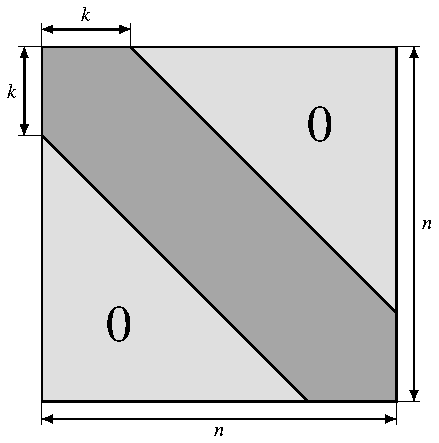
\includegraphics{chapters/60-linsys/images/bandmatrix.pdf}
\caption{Eine Bandmatrix ist eine $n\times n$-Matrix, deren Einträge
ausserhalb eines Bandes um die Diagonale verschwinden.
\index{Band}%
\label{buch:figure:bandmatrix}}
\end{figure}
Schematisch kann man eine solche Matrix wie in
Abbildung~\ref{buch:figure:bandmatrix} darstellen.

Der Gauss-Algorithmus braucht auch in einer Bandmatrix nicht die
volle Zahl von Operationen.
Bei der Pivotdivision müssen höchstens $2k+1$ Divisionen ausgeführt
werden.
\index{Pivotdivision}%
Danach sind genau $k$ Zeilenoperationen notwendig, um die Spalte
unter dem Pivotelement zu $0$ zu machen.
\index{Zeilenoperation}%
Dabei werden nur die Elemente in $2k+1$ Spalten modifiziert,
der Aufwand für jeden Schritt der Vorwärtsreduktion ist daher $(k^2)$.
\index{Vorwärtsreduktion}%
Nach $n$ Schritten wurde daher Rechenzeit $O(nk^2)$ aufgewendet.
\index{Rechenzeit}%
Beim Rückwärtseinsetzen werden in $n$ Iteration jeweils $k$ Zeilenoperationen
in genau zwei Spalten durchgeführt, es fallen also nur $O(nk)$
Operationen an.
\index{Rückwärtseinsetzen}%
Insgesamt sind also nur $O(nk^2)$ Operationen nötig, um ein Gleichungssystem
zu lösen, oder $O(n^2k^2)$ für eine Matrixinvertierung.
\index{Matrixinvertierung}%

Die Diskretisation einer partiellen Differentialgleichung in der Ebene
\index{partielle Differentialgleichung}%
\index{Differentialgleichung!partiell}%
mit finiten Differenzen
\index{finite Differenzen}%
(siehe auch Abschnitt~\ref{section:finite-differenzen})
führt auf natürlich Weise zu einem linearen
Gleichungssystem mit einer Bandmatrix mit $k\approx \sqrt{n}$.
Ein solches Gleichungssystem lässt sich mit Aufwand $O(n^2)$ statt 
$O(n^3)$ lösen.







